\documentclass[../main]{subfiles}
\usetikzlibrary{arrows.meta,decorations.markings,calc,patterns}

\begin{document}

\chapter{Efecto Magnus y aplicaciones del teorema de Bernoulli}

\section{Teorema de Bernoulli y sus aplicaciones}

El teorema de Bernoulli es un principio fundamental en la mecánica de fluidos que describe el comportamiento de un fluido moviéndose a lo largo de una línea de corriente. Este teorema tiene numerosas aplicaciones prácticas en la ingeniería y la física, desde el diseño de aviones hasta el funcionamiento de carburadores.

\info{Teorema de Bernoulli}{
El teorema de Bernoulli establece que en un fluido ideal\footnote{Un fluido hipotético que no tiene viscosidad} en régimen de circulación por un conducto cerrado, la energía que posee el fluido permanece constante a lo largo de su recorrido. Se expresa matemáticamente como:

\begin{equation}
P + \frac{1}{2}\rho v^2 + \rho g h = \text{constante}
\end{equation}

Donde:
\begin{itemize}
    \item $P$: Presión del fluido [Pa]
    \item $\rho$: Densidad del fluido [kg/m³]
    \item $v$: Velocidad del fluido [m/s]
    \item $g$: Aceleración debida a la gravedad [m/s²]
    \item $h$: Altura respecto a un nivel de referencia [m]
\end{itemize}
}

Esta ecuación muestra la relación entre la presión, la velocidad y la altura de un fluido en movimiento. Una consecuencia importante del teorema de Bernoulli es que, al aumentar la velocidad de un fluido, su presión disminuye, y viceversa. Este principio es fundamental para entender diversos fenómenos y aplicaciones tecnológicas.

\subsection{Efecto Magnus}

El efecto Magnus es un fenómeno físico observable en objetos en rotación que se mueven a través de un fluido. Este efecto es una aplicación directa del teorema de Bernoulli y tiene importantes implicaciones en diversos campos, desde el deporte hasta la ingeniería aeronáutica.

\info{Efecto Magnus}{
El efecto Magnus se produce cuando un objeto giratorio se mueve a través de un fluido. La rotación del objeto crea una diferencia de presión entre los lados opuestos del objeto, lo que resulta en una fuerza perpendicular a la dirección del movimiento.






\begin{equation}
F_M = \frac{1}{2}\rho A v^2 C_L
\end{equation}

Donde:
\begin{itemize}
    \item $F_M$: Fuerza de Magnus [N]
    \item $\rho$: Densidad del fluido [kg/m³]
    \item $A$: Área de referencia del objeto [m²]
    \item $v$: Velocidad relativa entre el objeto y el fluido [m/s]
    \item $C_L$: Coeficiente de sustentación (depende de la forma del objeto y su rotación)
\end{itemize}
}

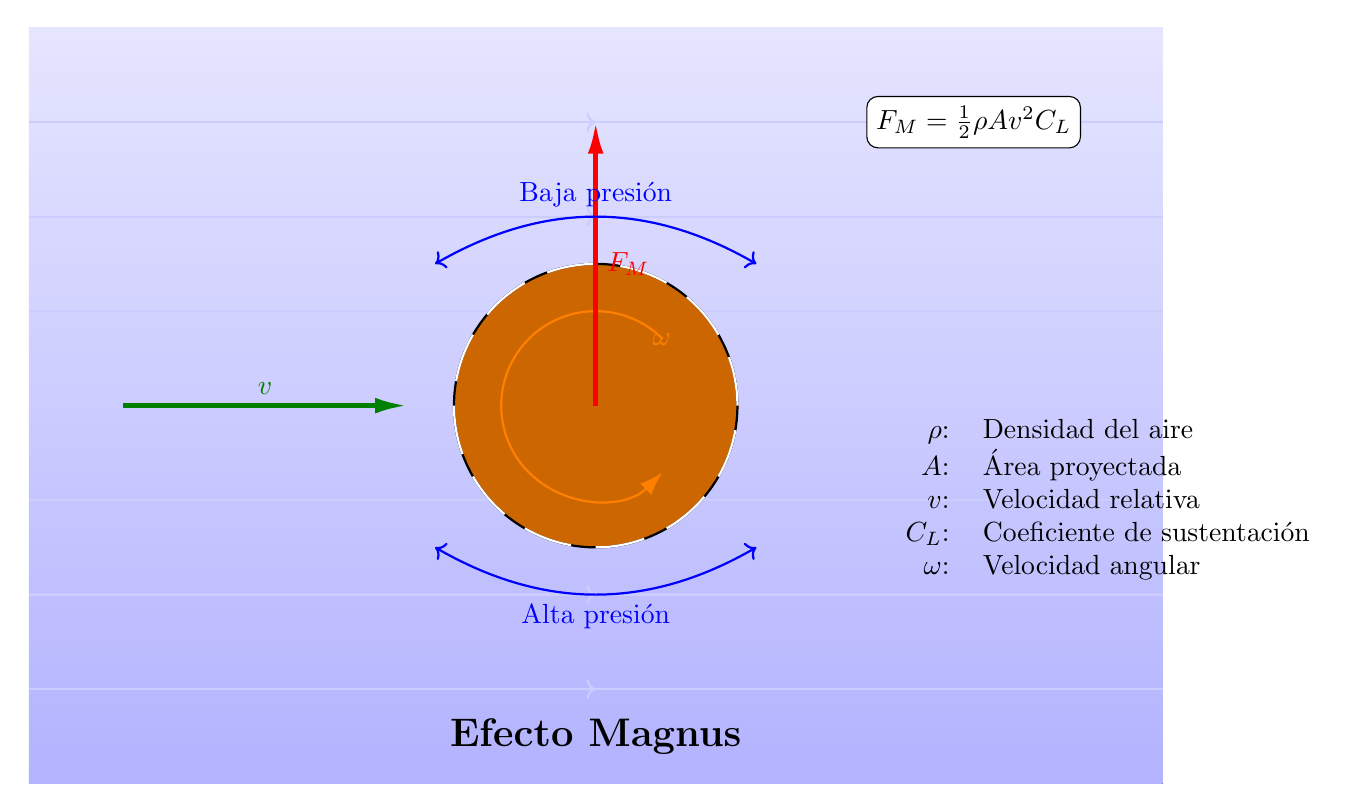
\begin{tikzpicture}[scale=1.2]
    % Definición de colores
    \colorlet{ballcolor}{orange!80!black}
    \colorlet{aircolor}{blue!20}
    \colorlet{forcecolor}{red}
    \colorlet{velocitycolor}{green!50!black}
    
    % Fondo
    \fill[top color=blue!10,bottom color=blue!30] (-6,-4) rectangle (6,4);
    
    % Flujo de aire
    \foreach \y in {-3,-2,...,3}
    {
        \draw[aircolor,thick,decoration={markings,mark=at position 0.5 with {\arrow{>}}},postaction={decorate}] (-6,\y) -- (6,\y);
    }
    
    % Pelota
    \fill[ballcolor] (0,0) circle (1.5);
    \draw[thick] (0,0) circle (1.5);
    
    % Patrón de rotación
    \foreach \angle in {0,30,...,330}
    {
        \draw[white,thick] ({1.5*cos(\angle)},{1.5*sin(\angle)}) arc (\angle:\angle+20:1.5);
    }
    
    % Flecha de rotación
    \draw[-{Latex[length=3mm,width=2mm]},thick,orange] (0,0) +(45:1) arc (45:315:1);
    \node[orange] at (0.7,0.7) {$\omega$};
    
    % Velocidad relativa
    \draw[-{Latex[length=4mm,width=2mm]},velocitycolor,ultra thick] (-5,0) -- (-2,0) node[midway,above] {$v$};
    
    % Fuerza de Magnus
    \draw[-{Latex[length=4mm,width=2mm]},forcecolor,ultra thick] (0,0) -- (0,3) node[midway,right] {$F_M$};
    
    % Líneas de presión
    \draw[<->,blue,thick] (-1.7,1.5) to[bend left] node[midway,above] {Baja presión} (1.7,1.5);
    \draw[<->,blue,thick] (-1.7,-1.5) to[bend right] node[midway,below] {Alta presión} (1.7,-1.5);
    
    % Ecuación de la fuerza de Magnus
    \node[draw,fill=white,rounded corners] at (4,3) {$F_M = \frac{1}{2}\rho A v^2 C_L$};
    
    % Variables
    \node[anchor=west] at (3,-1) {
        \begin{tabular}{rl}
            $\rho$: & Densidad del aire \\
            $A$: & Área proyectada \\
            $v$: & Velocidad relativa \\
            $C_L$: & Coeficiente de sustentación \\
            $\omega$: & Velocidad angular
        \end{tabular}
    };
    
    % Título
    \node[font=\Large\bfseries] at (0,-3.5) {Efecto Magnus};

\end{tikzpicture}


\ejemplo{Ejemplo del Efecto Magnus}{
Consideremos una pelota de fútbol que se patea con efecto. Al girar, la pelota crea una zona de alta presión en un lado y baja presión en el otro. Si la pelota gira en sentido horario visto desde arriba, se desviará hacia la derecha debido a la fuerza de Magnus.

Supongamos los siguientes datos:
\begin{itemize}
    \item Densidad del aire: $\rho = 1.225$ kg/m³
    \item Diámetro de la pelota: $d = 0.22$ m
    \item Velocidad de la pelota: $v = 25$ m/s
    \item Coeficiente de sustentación: $C_L = 0.2$ (valor típico para una pelota en rotación)
\end{itemize}

Calculamos el área de referencia: $A = \pi r^2 = \pi (0.11\text{ m})^2 = 0.038$ m²

Aplicando la ecuación:

\begin{equation}
F_M = \frac{1}{2} \times 1.225 \frac{\text{kg}}{\text{m}^3} \times 0.038 \text{ m}^2 \times (25 \frac{\text{m}}{\text{s}})^2 \times 0.2 = 2.91 \text{ N}
\end{equation}

Esta fuerza de 2.91 N perpendicular a la dirección del movimiento causa la curvatura en la trayectoria de la pelota.
}

\subsection{Aplicaciones del teorema de Bernoulli}

El teorema de Bernoulli tiene numerosas aplicaciones prácticas en la ingeniería y la vida cotidiana. A continuación, exploraremos algunas de estas aplicaciones:

\subsubsection{Chimeneas}

Las chimeneas utilizan el principio de Bernoulli para mejorar la extracción de humos y gases. 

\info{Funcionamiento de las chimeneas}{
En una chimenea, el aire caliente del interior es menos denso que el aire exterior frío. Esta diferencia de densidad causa un flujo ascendente. Además, el viento que sopla sobre la parte superior de la chimenea crea una zona de baja presión, lo que mejora aún más la extracción de humos.

La velocidad del viento en la parte superior de la chimenea se relaciona con la presión según la ecuación de Bernoulli:

\begin{equation}
P_1 + \frac{1}{2}\rho v_1^2 = P_2 + \frac{1}{2}\rho v_2^2
\end{equation}

Donde los subíndices 1 y 2 se refieren a las condiciones en la base y en la parte superior de la chimenea, respectivamente.
}

\subsubsection{Carburador}

El carburador es un dispositivo utilizado en motores de combustión interna para mezclar aire y combustible en la proporción adecuada. Su funcionamiento se basa en el principio de Bernoulli.

\info{Funcionamiento del carburador}{
En un carburador, el aire pasa por un estrechamiento llamado venturi\footnote{Sección estrecha de un tubo que causa un aumento en la velocidad del fluido y una disminución en su presión}. Según el teorema de Bernoulli, la velocidad del aire aumenta en esta sección, lo que resulta en una disminución de la presión. Esta baja presión succiona el combustible desde un depósito, mezclándolo con el aire.

La relación entre la velocidad y la presión en el venturi se puede expresar como:

\begin{equation}
P_1 - P_2 = \frac{1}{2}\rho (v_2^2 - v_1^2)
\end{equation}

Donde los subíndices 1 y 2 se refieren a las condiciones antes y en el venturi, respectivamente.
}

\subsubsection{Ala de avión}

El diseño de las alas de avión es una de las aplicaciones más conocidas del teorema de Bernoulli. La forma aerodinámica de las alas permite generar la sustentación necesaria para el vuelo.

\info{Sustentación en alas de avión}{
Las alas de avión tienen una forma asimétrica, con la parte superior más curvada que la inferior. Esto causa que el aire que pasa por encima del ala recorra una distancia mayor en el mismo tiempo que el aire que pasa por debajo. Según el teorema de Bernoulli, esta mayor velocidad en la parte superior resulta en una menor presión, creando una fuerza de sustentación hacia arriba.

La fuerza de sustentación se puede calcular aproximadamente como:

\begin{equation}
F_L = \frac{1}{2}\rho v^2 A C_L
\end{equation}

Donde:
\begin{itemize}
    \item $F_L$: Fuerza de sustentación [N]
    \item $\rho$: Densidad del aire [kg/m³]
    \item $v$: Velocidad del avión relativa al aire [m/s]
    \item $A$: Área de las alas [m²]
    \item $C_L$: Coeficiente de sustentación (depende del ángulo de ataque y la forma del ala)
\end{itemize}
}

\subsubsection{Alerón trasero de vehículo}

Los alerones traseros en vehículos de alta velocidad, como coches de carreras, utilizan el principio de Bernoulli para generar carga aerodinámica, mejorando la estabilidad y el agarre del vehículo.

\info{Funcionamiento del alerón trasero}{
El alerón trasero tiene una forma similar a un ala de avión invertida. Cuando el vehículo se mueve a alta velocidad, el aire que pasa por debajo del alerón se mueve más rápido que el aire que pasa por encima. Esta diferencia de velocidades crea una zona de baja presión debajo del alerón y una de alta presión encima, generando una fuerza hacia abajo (carga aerodinámica).

La fuerza de carga aerodinámica se puede expresar de manera similar a la sustentación en un ala:

\begin{equation}
F_D = \frac{1}{2}\rho v^2 A C_D
\end{equation}

Donde:
\begin{itemize}
    \item $F_D$: Fuerza de carga aerodinámica [N]
    \item $\rho$: Densidad del aire [kg/m³]
    \item $v$: Velocidad del vehículo [m/s]
    \item $A$: Área del alerón [m²]
    \item $C_D$: Coeficiente de arrastre (depende de la forma y ángulo del alerón)
\end{itemize}
}

\actividad{Responder el siguiente cuestionario}
\begin{enumerate}
\item ¿Cuáles son las tres formas de energía que componen la ecuación de Bernoulli?
\item ¿Cómo se relaciona la velocidad de un fluido con su presión según el teorema de Bernoulli?
\item ¿Qué es el efecto Magnus y en qué situaciones cotidianas podemos observarlo?
\item ¿Por qué las chimeneas son más eficientes en días ventosos?
\item ¿Cómo utiliza un carburador el principio de Bernoulli para mezclar aire y combustible?
\item ¿Por qué las alas de avión tienen una forma asimétrica?
\item ¿Cuál es la principal diferencia entre la función de un ala de avión y un alerón trasero de vehículo?
\item ¿Cómo afecta la densidad del aire a la fuerza de sustentación en un ala de avión?
\item ¿Qué papel juega el coeficiente de sustentación en la ecuación de la fuerza de Magnus?
\item ¿Cómo podría aplicarse el teorema de Bernoulli para explicar el funcionamiento de un atomizador de perfume?
\end{enumerate}

\actividad{Resolver los siguientes problemas}
\begin{enumerate}
\item Una pelota de béisbol con un diámetro de 7.3 cm se lanza con una velocidad de 40 m/s y un efecto que produce un coeficiente de sustentación de 0.3. Si la densidad del aire es 1.2 kg/m³, ¿cuál es la magnitud de la fuerza de Magnus que actúa sobre la pelota?
\item En un carburador, la presión en la sección más ancha es de 101.3 kPa y la velocidad del aire es de 10 m/s. Si la densidad del aire es 1.2 kg/m³, ¿cuál será la presión en el venturi si la velocidad del aire allí es de 60 m/s?
\item Un avión tiene alas con un área total de 90 m². Si vuela a una velocidad de 250 km/h a una altitud donde la densidad del aire es 1.0 kg/m³, y el coeficiente de sustentación es 0.8, ¿cuál es la fuerza de sustentación generada?
\item Un coche de carreras utiliza un alerón trasero con un área de 1.2 m². Si el coche viaja a 180 km/h y el coeficiente de arrastre del alerón es 1.1, ¿cuál es la fuerza de carga aerodinámica generada? Asuma una densidad del aire de 1.2 kg/m³.
\item Una chimenea tiene una altura de 10 m. Si la temperatura en la base es de 200°C y en la parte superior es de 100°C, ¿cuál es la diferencia de presión entre la base y la parte superior? Asuma que la densidad del aire caliente es 0.7 kg/m³ y la aceleración debida a la gravedad es 9.8 m/s².
\item Un tubo de Pitot en un avión mide una presión total de 105 kPa. Si la presión estática es 95 kPa, ¿cuál es la velocidad del aire? Asuma una densidad del aire de 1.1 kg/m³.
\item Una bola de golf con un diámetro de 4.3 cm se golpea con una velocidad inicial de 70 m/s. Si el coeficiente de sustentación debido a su rotación es 0.1 y la densidad del aire es 1.2 kg/m³, ¿cuál es la magnitud de la fuerza de Magnus?
\item En un sistema de ventilación, el aire fluye a través de un conducto que se estrecha de un diámetro de 30 cm a 15 cm. Si la velocidad en la sección más ancha es de 5 m/s, ¿cuál será la velocidad en la sección más estrecha?
\item Un alerón de un coche de Fórmula 1 genera una fuerza de carga aerodinámica de 7000 N cuando el coche viaja a 300 km/h. Si el área del alerón es de 1.5 m² y la densidad del aire es 1.2 kg/m³, ¿cuál es el coeficiente de arrastre del alerón?
\item Una bomba de agua eleva agua desde un depósito a 5 m por debajo del nivel del suelo hasta un tanque 15 m por encima del suelo. Si la velocidad del agua en la tubería es de 2 m/s, ¿cuál es la presión que debe suministrar la bomba para vencer la diferencia de altura? Asuma que la presión en ambos extremos es la atmosférica y que la densidad del agua es 1000 kg/m³.
\end{enumerate}

\end{document}